\chapter{Implementierung}
Nun da die Grundlagen gelegt sind können wir anfangen zu untersuchen wie ein LSTM Netz mit Events umgeht. Wir betrachten dazu das Bouncing Ball Szenario, da es klare Events hat und sich dadurch auch gut segmentieren lässt. Zur Implementation wurde JANNLab (Otte et al. 2013), ein Java Framework für Neuronale Netze verwendet \cite{bib:jannlab}. Dieses Kapitel soll die im Zuge dieser Arbeit verwendeten Techniken erklären, die betrachteten Testfälle definieren und aufzeigen wie die im nächsten Kapitel beschriebenen Erkenntnisse gewonnen wurden, sowie welche Probleme sich dabei in den Weg gestellt haben.

\section{Das Bouncing Ball Szenario}
Das Bouncing Ball Szenario beschreibt einen Ball, der gleichförmig durch die Ebene gleitet bis er an entsprechenden Begrenzungen abprallt. Wir haben die 1- und die 2-dimensionale Version verwendet.

Im 1D Fall haben wir einen Ball ohne Ausdehnung (also eigentlich ein Punkt aber diese Unterscheidung ist für unsere Zwecke irrelevant) mit einer Position $ x_{b} $ und einer konstanten Geschwindigkeit $  v$. Dieser springt zwischen den Grenzen $ x_{1}=-1 $ und $ x_{2}=1 $ hin und her, also immer wenn die Position des Balls eine der Grenzen annimmt, wird die Geschwindigkeit invertiert $ v := -v $. Also genau so wie man es sich vorstellt. Der 1D Fall unterteilt sich also in 2 Ereignisse, die "Bewegung nach links" und die "Bewegung nach rechts", wenn man das Bouncen zwischen -1 und 1 als Bewegung auf einer horizontalen Linie nimmt.

Der 2D Fall funktioniert analog, der Ball hat eine Position $ (x_{b}/y_{b}) $, eine konstante Geschwindigkeit $ (v_{x}/v_{y}) $, welcher nun zwischen den 4 Grenzen $ x_{1}=-1 $ und $ x_{2}=1 $, $ y_{1}=-1 $ und $ y_{2}=1 $ hin und her springt. Nimmt nun eine Koordinate des Balls eine der Grenzen an wird die entsprechende Koordinate invertiert, also $ (v_{x}/v_{y}) = (-v_{x}/v_{y}) $ beziehungsweise $ (v_{x}/-v_{y}) $. Der 2D Fall unterteilt sich also in 4 Ereignisse, die "Bewegung in Richtung oben-rechts", etc. wenn man das Bouncen zwischen dem Quadrat von (-1/-1) und (1/1) im 2-dimensionalen als Bewegung in einer stehenden Ebene nimmt.

Das 1D-Szenario habe ich hauptsächlich verwendet um mich einzuarbeiten und zurechtzufinden, da es unter anderem mit weniger Neuronen erlernt werden kann und so die Aktivierungen der einzelnen Gates auch übersichtlicher sind. Der Grund warum das 1D-Szenario auch für diese Ausarbeitung wichtig ist, ist das unter Hinzunahme der Zeitachse aussagekräftige Diagramme erstellt werden können, anhand derer einige Trainingseffekte und Verläufe veranschaulicht werden können. Entsprechende Analysen konnten vom 2D-Fall auch gemacht werden, wenn man sah wie sich eine Linie oder ein Ball mit Verzögerung entsprechend über den Bildschirm bewegt, die resultierenden Bilder sind jedoch eher unübersichtlich. Das 2D Szenario hingegen ist das für unsere Untersuchungen interessantere, da es mehr Events gibt, die auch in komplexernen Beziehungen zueinander stehen. In Abbildung \ref{img:1dvs2d} sieht man jeweils 2 Beispiele, zu dem genauen Aufbau des dazu benutzten LSTM Netzes kommen wir in der folgenden Sektion.
\begin{figure}
	\centering
	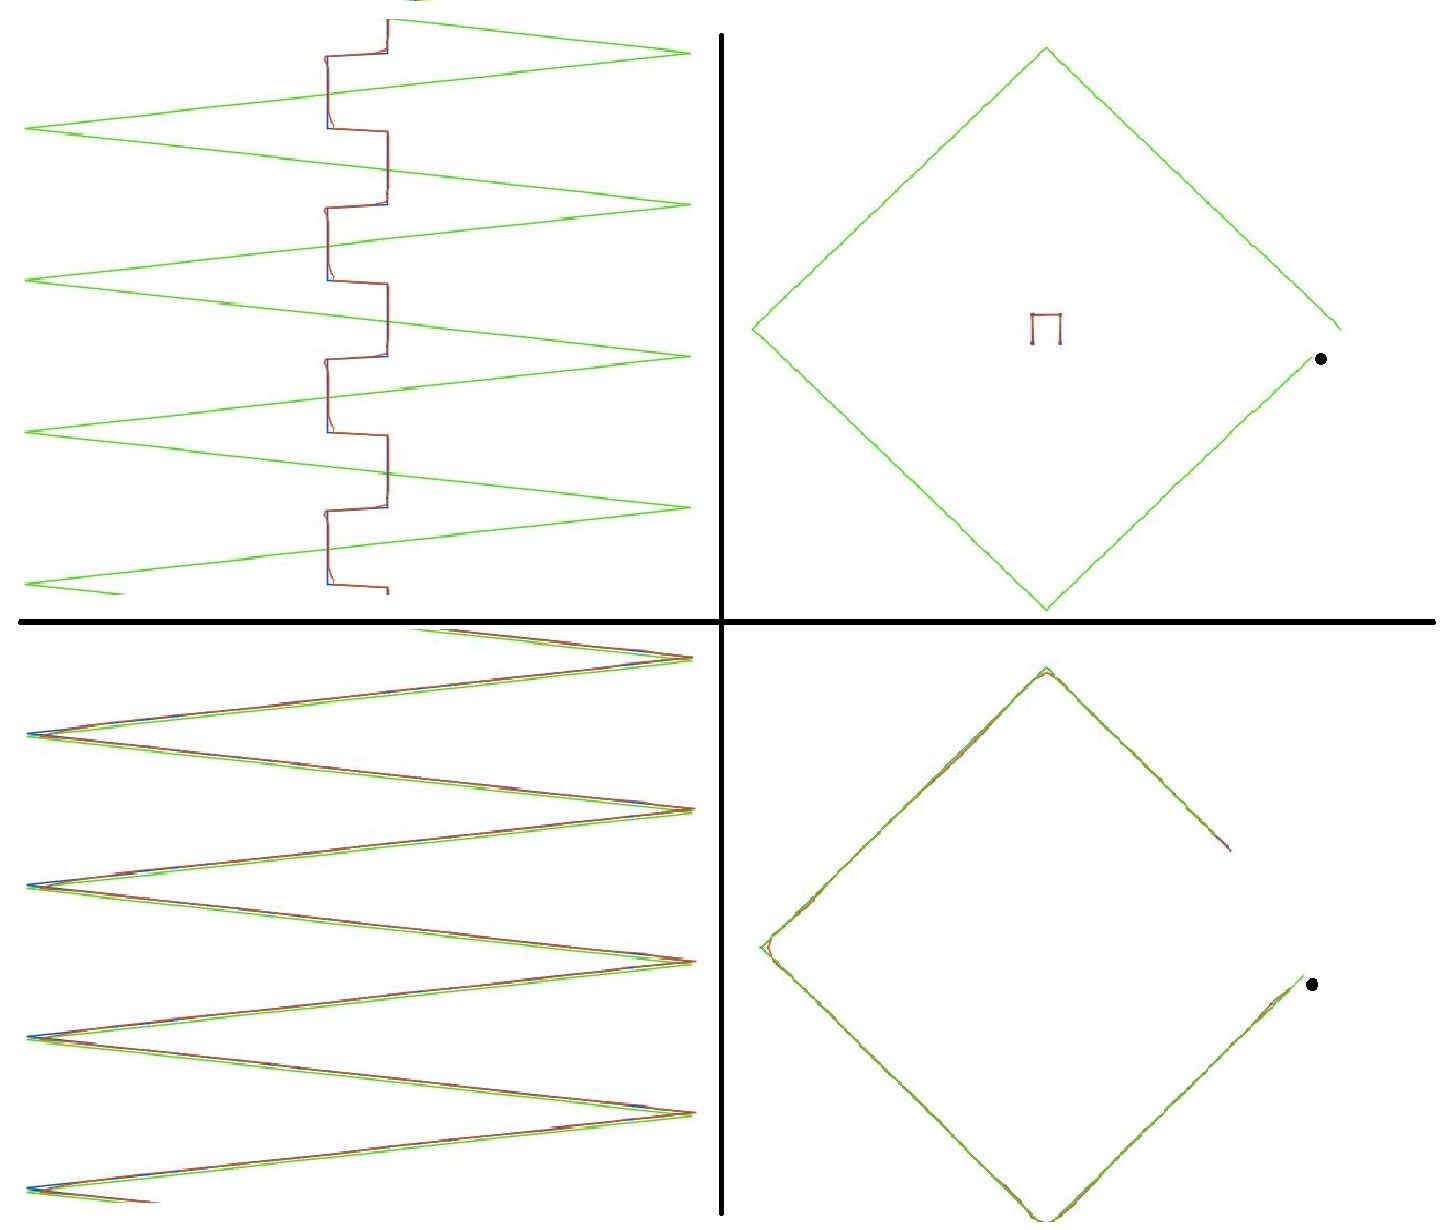
\includegraphics[width=0.9\textwidth, height=370px]{pics/1dvs2d.jpg}	
	\caption{4 Versionen des Bouncing Ball Szenario erlernt durch LSTM Netze. Zu sehen sind der Netzinput (grün), der Netzoutput (rot) und das Trainingsziel (blau). Links sieht man 2 Beispiele des 1D Falls, zur besseren Veranschaulichung sind die Daten nach den Zeitschritten vertikal versetzt. Rechts sieht man 2 Beispiele des 2D Falls, die Abbildung zeigt jeweils den Verlauf des Balls bis kurz vor dem vollenden einer Runde, um Überlagerungen in der Abbildung zu vermeiden. Der Startpunkt ist durch den schwarzen Punkt gekennzeichnet. In den jeweils oberen Fällen wurde als Netzinput die Position des Balles und als Trainingsziel die Geschwindigkeit des Balles für den nächsten Schritt. In den jeweils unteren Fällen wurde als Netzinput die Position des Balles und als Trainingsziel die vorauszuberechnende nächste Position des Balles.}
	\label{img:1dvs2d}
\end{figure}

\section{Parameter und Testfälle}
Für unser LSTM-Netz haben sich folgende Parameter als sinnvoll erwiesen:
\begin{description}	\item[Aktivierungsfunktionen:]\hfill \\ 
	Zur Ansteuerung der Gates der LSTM-Zellen im Hiddenlayer werden Neuronen mit \textit{Tangens hyperbolicus} als Aktivierungsfunktion verwendet. Für das Outputlayer wird zur Aktivierung die lineare Funktion verwendet, da die Position des Balles gleichverteilt Werte zwischen -1 und 1 annimmt, soll unser Netzoutput dasselbe tun. Anfangs war für das Outputlayer per Defaultoption die \textit{sigmoid}-Funktion zur Aktivierung eingestellt, deren Bild aber nur von 0 bis 1 reicht. Das hatte natürlich nicht funktioniert und für Verwirrung gesorgt, warum denn nur die Hälfte des Problems erlernt wird.  
	\item[Trainingsoptimierung:]\hfill \\ 
	Als Optimierungsmethode für das Traing wurde die Adaptive Moment Estimation Methode(ADAM), also eine adaptive Momentumsschätzung, verwendet. Diese baut die übliche Lernmethode mit Lernrate und Momentumrate dahingehend aus, dass diese durchgehend angepasst werden, um noch schneller zu genaueren Ergebnissen zu kommen. Hierzu wurden die Standard Parameter verwendet, also $ \beta_{1}=0.9, \beta_{2}=0.99 $ und $ \epsilon = 10^{-8}$. Wobei $ \beta_{1} $ und $ \beta_{2} $ die Abklingraten des Einflusses der vergangenen Momenti auf den jetzigen Zeitschritt sind. Sind sie Nahe 1, klingt der Einfluss langsamer ab. $ \epsilon$ ist ein glättender Term, der Division durch 0 verhindert. \cite{bib:adam} Es wurde für Debugging-Zwecke an diesen Werten herumgespielt, dadurch wurden aber nie sichtlich bessere Ergebnisse erzielt.
	\item[Netzgröße:]\hfill \\ 
	Die passende Netzgröße ist fallabhängig, in Abbildung \ref{img:1dvs2d} z.B. wurden für die 1D Fälle 1-2-1 Netze verwindet (also 1 Inputneuron, 1 Hiddenlayer mit 2 Neuronen und 1 Outputneuron), für die 2D Fälle 2-4-2 Netze. An anderer Stelle werden andere Netzgrößen verwendet, dann wird das dort, falls relevant, auch nochmal aufgegriffen.
	\item[Außerdem:]\hfill \\
	Alle Layer sind mit Bias-Unit, um mit möglichst wenig Neuronen möglichst viel Funktionalität zu erreichen, damit deren Analyse wiederum möglichst ausgiebig verläuft. Peepholes \cite{bib:lstm2} wurden getestet, hatten in diesem Beispiel keinen sichtbaren Effekt auf das Training und wurden dann weggelassen.  
\end{description}
Außerdem werden verschiedene Testfälle mit verschiedenen Intentionen betrachtet, die ich an dieser Stelle vorgreifend definieren möchte. Es wurde mit fast allen Kombinationen experimentiert:
\begin{description}
	\item[Verschiedene Inputs:] \hfill \\
	\begin{itemize}
		\item Position: Der Standard Input
		\item Noisy Position: Hier wird für den Input auf die Position des Balles noch ein zufälliger Wert zwischen -0.02 und 0.02 hinzu addiert, das Trainingsziel bleibt davon aber unbetroffen. Dieses "rauschen" soll das Netz dazu zwingen, eine innere Repräsentation von der Position des Balles zu haben, anstatt stur auf den Input einen konstanten Wert (die Geschwindigkeit) aufzuaddieren. Tatsächlich kann hier beobachtet werden, wie schon bei geringerer Epochenzahl das Bounce-Verhalten des Balles schneller erlernt wird.
		\item Null: Hier werden im 1. Schritt eine 1, dann aber nur noch 0-en in das Netz gespeist. Der Gedanke hierbei ist, das das Netz eine vom Input unabhängige Repräsentation des Balles hat, die sich auch als solche analysieren lassen kann. Im Standardfall mit fixer Startposition und Startgeschwindigkeit hat dies gut funktioniert, im zufälligen Fall natürlich nicht, das Netz kann ohne Input ja die anderen Position und Geschwindigkeit nicht kennen. Experimente mit einer "Lern-Phase", also das z.B. 100 Zeitschritte als Input die Position des Balles gegeben wird, bis das Netz ein Model von der Bewegung aufgebaut hat und ab dann den Input wegzulassen, schlugen fehl. 
		\item Geschwindigkeit: Ein Kompromiss zwischen dem Netz direkt die Position zu verraten und ihm keine Information zu liefern. Wichtig ist zu beachten, dass die Geschwindigkeit im Input sich unterscheidet von der Geschwindigkeit im Output indem sie einen Zeitschritt nach hinten versetzt ist. Sonst müsste das Netz auf die Position wirklich nur die Geschwindigkeit aufaddieren und müsste sonst keine Repräsentation des ganzen haben. Die Hoffnung war so auch die Fälle mit zufälligen Geschwindigkeiten zu erlernen (die Startposition muss hierfür natürlich fix sein), aber trotzdem das Modell unabhängiger vom Input zu haben. Dieser Fall hätte eine Repräsentation der Position des Balles gefordert und auch ein sauberes Handling der Eventgrenzen, da einfach nur Schritte Zählen nicht gereicht hätte, da bei verschiedenen Geschwindigkeiten die Events nach unterschiedlich vielen Schritten auftreten. Am vielen Konjunktiv in diesem Abschnitt merkt man aber, das dieser Trainingsfall leider nicht geklappt hat und es hat sich auch nicht mehr aufgeklärt was am Training hätte geändert werden müssen, um diesen Fall zu erlernen. Es wurden verschiedene fixe Startpunkte getestet, es wurden nur kleine Varianzen in der Geschwindigkeit getestet, der Output, die nächste Position des Balles, hat sehr schnell sehr falsches Verhalten aufgezeigt, wie z.B. in Abbildung \ref{img:chaos}.
	\end{itemize}

	\item[Verschiedene Trainingsziele:] \hfill \\
	\begin{itemize}
	
	\item Nächste Position: Das Standard Trainingsziel.
	\item Geschwindigkeit: Da die Geschwindigkeit bis auf Vorzeichen konstant ist, kann sich das Netz hier darauf konzentrieren zu klassifizieren, in welchem Ereignis, also Bewegungsabschnitt es sich befindet, also ob sich der Ball momentan z.B. nach links oben bewegt.  
	\item Nächstes Event: Es wurde auch getestet wie sich das Netz verhält wenn es selbst vorhersagen soll, welches Event als nächstes ansteht. War erfolgreich auch bei zufälligen Startposition und Geschwindigkeiten, was aber nicht weiter Überraschend ist, das sich das LSTM Netz auf ein lineares Problem, welche Grenze als nächstes getroffen wird, trainieren lässt. Auch aus den Aktivierungen im Netz konnte nichts interessantes gefolgert werden, weswegen das nächste Event als Trainingsziel nicht mehr aufgegriffen wird. 
	
\end{itemize}
	\item[Startposition und Geschwindigkeit:]\hfill \\
	\begin{itemize}
		\item Feste Startposition und Geschwindigkeit: Der Standard Fall, leicht zu erlernen. Der Ball wird so gesendet, dass er jede Grenze in der Mitte trifft und die Flugbahn wieder ein Quadrat beschreibt, wie z.B. in Abbildung \ref{img:1dvs2d} rechts. Dadurch ist das Trainingsziel aber auch immer dieselbe Zahlenfolge, und kann (und wird auch) auf andere Weise gelernt als die Eventgrenzen sauber zu lernen. Das Netz kann eine periodische Struktur erlernen, die gelernt hat das z.B. bei einer Geschwindigkeit von 0.1 alle 20 Schritte eine Eventgrenze vorliegt und die Geschwindigkeit invertiert werden muss. Oder aus dieser periodischen Struktur werden direkt die Netzausgaben generiert und eine Repräsentation des Bewegung des Balles wird komplett Übergangen. 
		
		Außerdem ist im 2D Version in diesem Fall die Ereignisabfolge immer dieselbe, was die Vorhersage des nächsten, bzw. die Einteilung des derzeitigen Ereignisses, nicht nur sehr vereinfacht, sondern auch entweder unabhängig von der derzeitigen Geschwindigkeit des Balles oder von der derzeitigen Position des Balles macht. Also um zu wissen, dass der nächste Bounce an der unteren Grenze erfolgt, genügt entweder das man sich gerade um Quadranten unten rechts befindet, oder das die Geschwindigkeit die Richtung nach unten-links hat. Im Allgemeinen ist dies aber nicht der Fall. 
		\item Zufällige Startposition und Geschwindigkeit: Um zu umgehen, dass das Netz das Problem auf Basis einer inneren periodischen Struktur erlernt, werden mehrere Testsätze (Größenordnung 100 Stück) mit zufälligen Startpositionen und Geschwindigkeiten generiert. Das Netz wird über alle trainiert. So haben die verschiedenen Fälle ihre Ereignisgrenzen in verschiedenen Abständen und das Netz wird dazu gezwungen das Bounce Verhalten an den Eventgrenzen zu erlernen. Das Problem hierbei war aber das die Definition des Bounceverhalten unklar war. Gewünscht ist natürlich, dass z.B. die Eventgrenze x=1 erreicht, aber nicht überschritten wird, da an ihr abgeprallt werden soll. Durch die Diskretisierung unser Zeitschritte und die zufällige Wahl von Position und Geschwindigkeit, wird die Grenze jedesmal überschritten und jedesmal um einen anderen Wert. Hat der Ball zum Beispiel die Position 0.95 und Geschwindigkeit 0.15, wird er er im nächsten Schritt die Position 1.1 haben, beim überschreiten der Grenze die Ereignisgrenze erreichen und umkehren. Den Bounce dann zu definieren, wenn im nächsten Schritt die Grenze überschritten werden würde, scheint noch willkürlicher, da dies manchmal bei 0.8, manchmal bei 0.99 ist. Die korrekte Berechnung, welche Position der Ball im kontinuierlichen Fall bis zum nächsten Zeitschritt erreicht hat, wäre die sinnvollste Definition. Also im obigen Beispiel mit der Position 0.95 und der Geschwindigkeit 0.15, bewegt der Ball sich 0.05 bis zur Grenze und die verbleibenden 0.10 wieder zurück, ist beim nächsten Zeitschritt also bei 0.9. Wurde getestet, konnte aber vom Netz nicht ohne weiteres erlernt werden. Es bleibt also bei der Definition, dass ein Bounce ausgeführt wird, wenn eine Grenze überschritten wird. Vermutlich leidet aber die Genauigkeit des Netzes beim Simulieren des Bounces darunter, dass der Bounce nicht an der Grene x=1, sondern in einem kompletten Bereich, abhängig von der Geschwindigkeit Varianz, zum Beispiel zwischen 1.0 und 1.999, ausgeführt wird. Daher wurde folgender Ansatz weiter verfolgt:
		\item Zufällige Auswahl aus vorgegebenen Startpositionen und Geschwindigkeiten: Ein Kompromiss aus den beiden anderen Varianten. Es werden geeignete Startpositionen und Geschwindigkeiten vorgegeben, sodass auch bei der diskreten Berechnung der Positionen zu den Zeitschritten, die Ereignisgrenzen immer exakt erreicht werden, anstatt sie zu überschreiten. Eine der Möglichkeiten und auch von uns verwendete ist hierzu, die Startposition $ x_{0} \in \{-0.9,-0.8, ... ,0.8,0.9\} $ und die Startgeschwindigkeit $ v_{0} \in \{-0.1,-0.05,0.05,0.1\} $ zu wählen. Im 2D Fall natürlich jeweils 2 wählen, pro Koordinate eine wie z.B. in Abbildung \ref{img:fb}. Außerdem wurde für den 2D Fall noch genau die Teilmenge betrachtet, deren Flugbahn wieder genau auf dem Standard Quadrat wie in Abbildung \ref{img:1dvs2d} rechts liegt, nur eben in beide Richtungen und in 2 verschiedenen Geschwindigkeiten durchlaufen. 
		
		Nun hat man beim erstellen der Testsätze zwar, wenn man auf die Position des Balles 100 mal eine Geschwindigkeit auffadiert um jeweils die neue Position zu erhalten, ein Computernumerisches Problem, dass eventuell anstatt genau die Eventgrenze x=1 zu erreichen, ein Wert knapp darunter, z.B 0.9999 berechnet wird und man die Grenze wieder überschreiten würde. Ist man sich dessen aber bewusst geworden, kann man es leicht, durch das einbauen eines kleinen Thresholdes um die Ereignisgrenzen, umgehen. 
	\end{itemize}
	\item[Feedback:]\hfill \\
	Die Rück-Einspeisung (engl. Feedback) des Outputs $ y_{t} $ des Netzes als Input im nächsten Zeitschritt $ x_{t+1} $ hat mehrere Effekte auf Training und Verhalten des Netzes. Sinnvoll ist dies natürlich nur, wenn der Output des Netzes die Informationen für einen geeigneten Input enthält. Genutzt haben wir dies für die Position des Balles als Input (bzw. auch Noisy Position) und für den Output entweder die nächste Position des Balles, dann kann der Output direkt als Input für den nächsten Zeitschritt verwendet werden $ x_{t+1} = y_{t} $, oder mit Geschwindigkeit im nächsten Zeitschritt als Output, dann wird die bestimmte Geschwindigkeit auf die letzte Position aufaddiert und als Input genommen  $ x_{t+1} = x_{t}+y_{t} $. Hierzu werden in den ersten 100 Zeitschritten wie gewohnt der Input aus dem jeweiligen Testsatz genommen, sodass sich das Netz gut auf den jeweiligen Fall einstellen kann. Nach dieser Lernphase beginnt man mit der Rück-Einspeisung des Outputs. Die Feedback-Methode wurde wie folgt mit den beschriebenen Effekten eingesetzt: \hfill \\
	\begin{itemize}
		\item Genaueres Training: \hfill \\
		 Der Effekt der in Abbildung \ref{img:chaos} beschrieben ist, das wenn das Netz die Position des Balles selbst lenkt kleine Abweichungen große Fehler erzeugen, kann sowohl ein Nachteil als auch für uns jetzt ein bewusst genutzter Vorteil sein. Wird Feedback schon beim Training verwendet, wird das Netz direkt gezwungen genaue Ausgaben zu erzeugen. Das Trainingsziel kann so deutlich schneller erreicht werden. 
		\item Überprüfen eines bereits trainierten Netzes: \hfill \\
		 Hat man ein Netz trainiert und wendet dann im Testfall die Feedback Methode an, sieht man, wie z.B. in Abbildung \ref{img:1d1}, recht schnell wie gut das Training ist und wie sehr das Problem wirklich erlernt oder nur eine passende Annäherung gefunden wurde. 
		\item Konsistenz mit innerer Repräsentation: \hfill \\
		 Hat man ein Netz welches intern eine Repräsentation des Modells hat, z.B. die Position des Balles selbst speichert und diese abhängig vom Input aktuallisiert, kann es zu einem Zitter-Effekt kommen, wie man ihn in Abbildung \ref{img:fb} sieht. Eine Abweichung in der gespeicherten Position des Balles im Gegensatz zur tatsächlichen Position die per Input reinkommt, wurde erlernt wieder korrigiert zu werden. Gehen die Abweichungen mal in beide Richtungen, sieht man dieses Zittern. Nutzt man hingegen die Feedback Methode werden diese Korrekturen nicht vorgenommen, da der Input selbst auch vom Netz generiert wurde. Dies ist je nach Anwendung natürlich ein Nachteil, da Abweichungen sich aufaddieren und über die Zeit das Endergebnis ein ganz anderes sein wird. Andererseits, wenn es einem wie in unserem Fall nicht um die Bestimmung der Endposition des Balles nach 300 Schritten, sondern um das Verhalten auf dem Weg dorthin geht, erhält man mit der Feedback Methode zueinander konsistente Zwischenergebnisse, wie z.B. in Abbildung \ref{img:fb} zu sehen.
	\end{itemize}
	Feedback funktioniert gut für die 1D Fälle und für die 2D Fälle, wo die Laufbahn des Balles auf dem Hauptquadrat bleibt, leider aber nicht für die Fälle wo der Ball sich frei bewegt. Es wurden mit verschieden langen Findungsphasen, also Phasen in denen der Input noch aus dem Testset kommt experimentiert, auch zum Beispiel 90\% der gesammten Simulationslänge. Es wurde getestet wenn man das Feedback erst nach einer hohen Epochenzahl an das Netz langsam heranführt, also das Netz erst ohne Feedback trainiert und erst wenn das Netz gute Ausgaben liefert, dann erst nur die letzten Zeitschritte mit Feedback simuliert und so das Netz langsam daran heranführt, auch ohne Erfolg. Es wurde mit einem Mittelwert aus dem vorgegeben Input und dem Input aus Feedback, also dem dem eigenen vergangenen Output, experimentiert, und auch mit verschiedenen Anteilen hier, auch einem der sich über höhere Epochenzahl anpasst, auch ohne Erfolg. Der Effekt aus Abbildung \ref{img:chaos} ist wohl zu stark, das auch gute Annäherungen des Bounce-Verhaltens doch über die Zeit zu großen Abweichungen führen und diese dann nicht als gute Annäherungen erkannt werden. 
	
	Das Netz Online zu trainieren wäre für diesen speziellen Fall wohl die Lösung gewesen, d.h. den Input und vorallem das Trainingsziel nicht in Testsätzen im vorneherein zu berechnen und zu definieren, sondern auch das Trainingsziel in jedem Zeitschritt agil zu berechnen, also die aktuelle Geschwindigkeit aus den beiden vorherigen Positionen zu bestimmen, sodass Abweichungen in der Richtung auch vom Trainingsziel berücksichtigt werden. Ein solches Online-Training hätte aber eine komplette Umstrukturierung der bestehenden Implementierung vorausgesetzt, was an dieser Stelle nicht durchgeführt wurde, da die Tatsache ob das LSTM Netz mit Feedback trainiert wurde oder nicht, wohl keinen Einfluss darauf hat wie sich die LSTM Zellen im Bezug auf die Eventgrenzen verhalten, was der eigentliche Kern dieser Arbeit ist. 
\end{description}

\begin{figure}
	\centering
	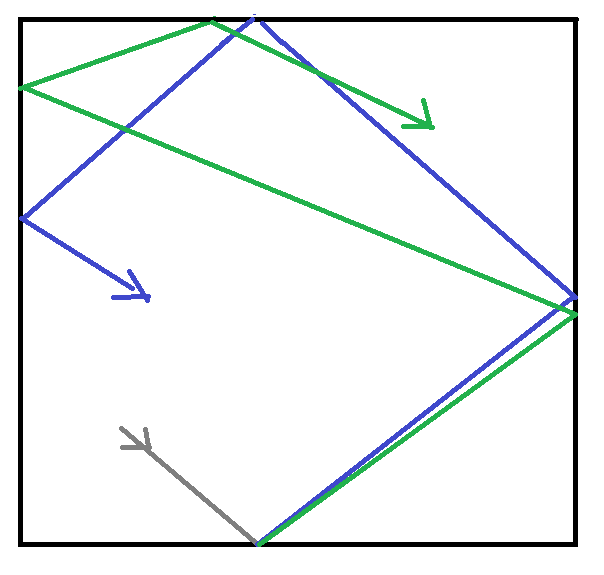
\includegraphics[width=0.5\textwidth, height=160px]{pics/chaos.png}	
	\caption{Chaostheorie im Bouncing Ball Szenario: Kleine Abweichungen im Bounce Verhalten haben große Auswirkungen auf den weiteren Flug des Balls. Dies ist der Grund für Probleme beim Offline Training von Fällen, wo das Netz die Position des Balles selbst lenkt, da sehr gute Annäherungen des korrekten Bounce Verhaltens trotzdem große Fehler über Zeit erzeugen, werden also nicht als gute Annäherungen erkannt.}
	\label{img:chaos}
\end{figure}
\begin{figure}
	\centering
	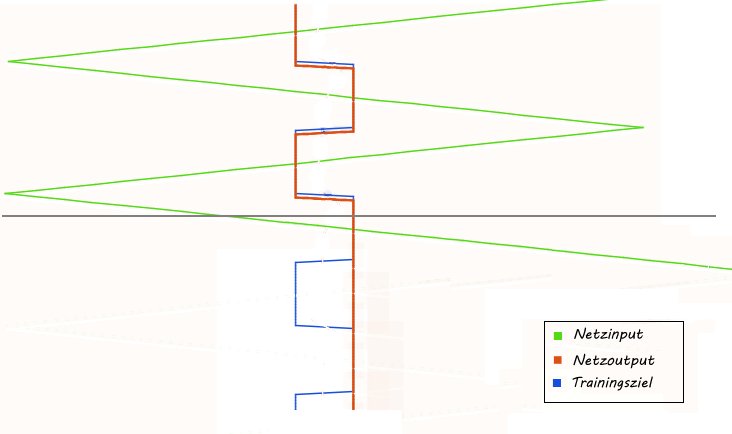
\includegraphics[width=0.5\textwidth, height=160px]{pics/1D1.png}	
	\caption{1D Fall mit der Geschwindigkeit als Trainingsziel erlernt von einem 1-1-1 Netz. Trainiert ohne Feedback, zur Überprüfung des Trainings dann hier im Bild verwendet, setzt auf Höhe der horizontalen grauen Linie an. Man sieht, dass das Netz das Bounce Verhalten nicht erlernt hat und als Abschätzung der nächsten Geschwindigkeit die vergangene Geschwindigkeit verwendet. Der Output ist so zum Trainingsziel um einen Zeitschritt versetzt. Setzt dann aber das Feedback ein und das Netz steuert den Input selbst, läuft dieser mit konstanter Geschwindigkeit davon. Außerdem ist hier der Nutzen von Feedback als Testmethode des Trainings gut veranschaulicht.}
	 \label{img:1d1}
\end{figure}
\begin{figure}
	\centering
	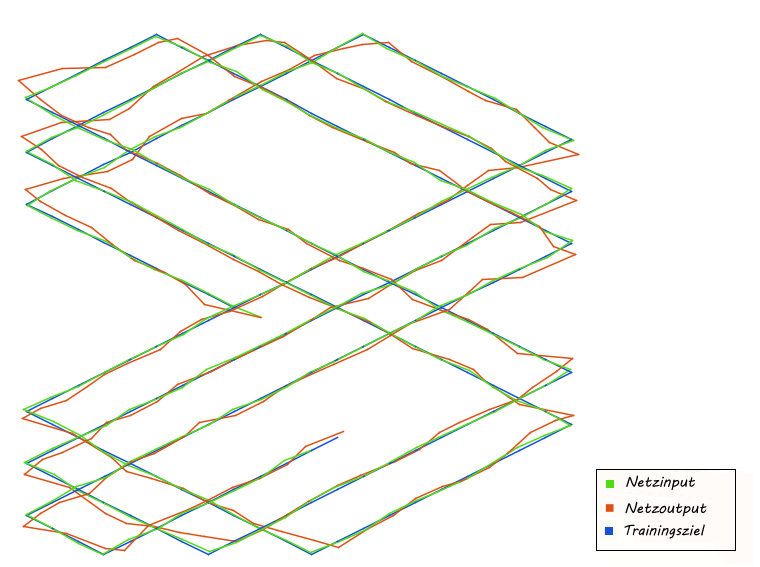
\includegraphics[width=0.6\textwidth, height=160px]{pics/fb.png}	
	\caption{2D Fall mit zufällig gewählter Startposition und Geschwindigkeit. Auch wenn das Ergebnis sehr nah am Trainingsziel ist, sieht man hier sehr deutlich das beschriebene Zittern, das sich durch anwenden der Feedback-Methode vermeiden lässt.}
	\label{img:fb}
\end{figure}
\begin{figure}
	\centering
	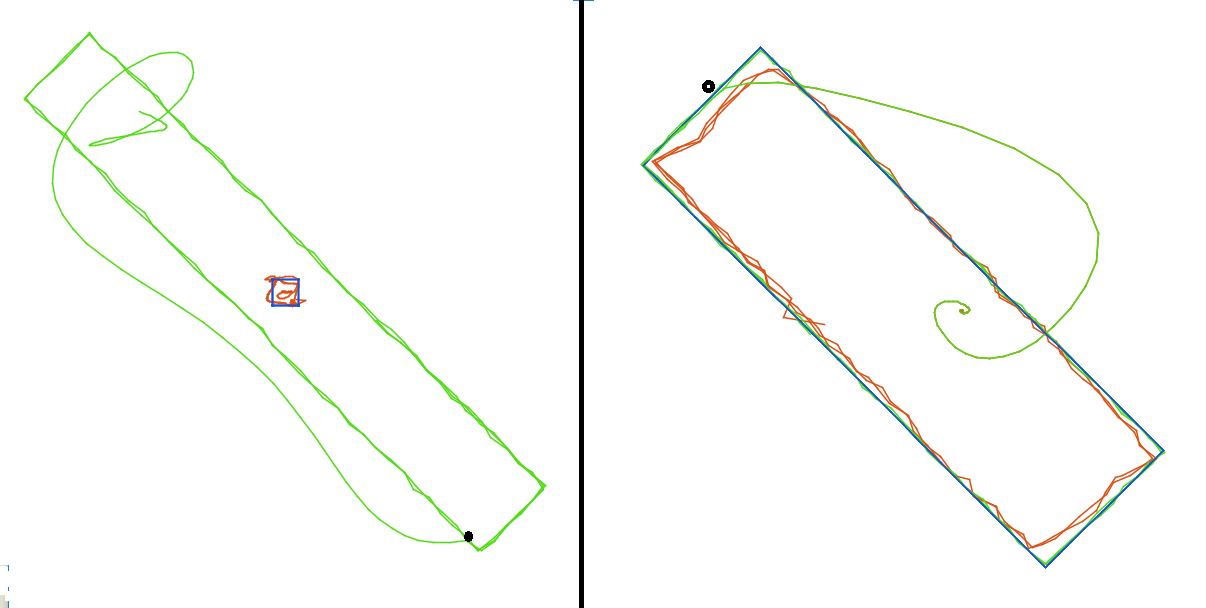
\includegraphics[width=0.9\textwidth, height=160px]{pics/fb2.png}	
	\caption{2 Fälle trainiert mit je einem 2-16-2 Netz mit Feedback. Links als Trainingsziel die Geschwindigkeit, Rechts als Trainingsziel die nächste Position. Feedback setzt nach der halben Simulationslänge ein, hier mit schwarzem Punkt markiert. Auch wenn das Ergebnis offensichtlich weit vom Trainingsziel entfernt ist, sieht man die glättende Wirkung der Feedback Methode.}
	\label{img:fb2}
\end{figure}



